%% zusammenf.tex
%% $Id: zusammenf.tex 61 2012-05-03 13:58:03Z bless $
%%

\chapter{Zusammenfassung und Ausblick}
\label{ch:Zusammenfassung}
%% ==============================
Zusammenfassend l"asst sich also sagen, dass es viele M"oglichkeiten heute gibt, Daten zu speichern. Die einen sind praktischer, die anderen etwas unpraktischer.
Der meist genutzte Massenspeicher ist im Moment wohl die Festplatte, seine Entwicklung war rasant –
\begin{figure}[ht]
				\centering
				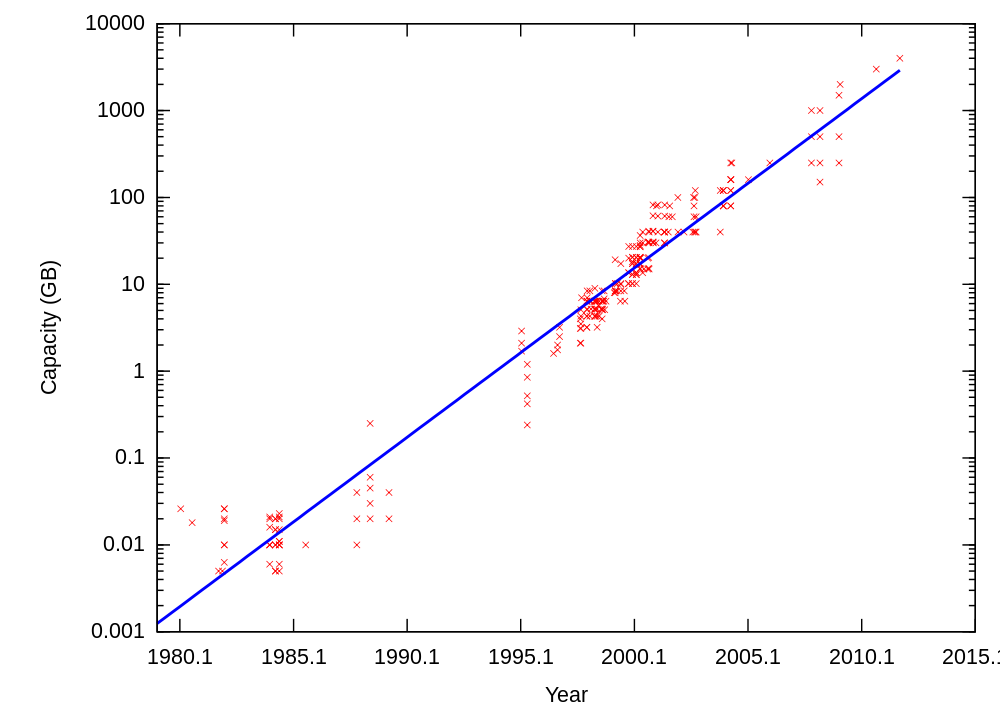
\includegraphics[width=0.7\textwidth]{images/kapazit} 
				\caption[Entwicklung Speicherkapazit"at Fesplatte in halblogarithmischer Skalierung \cite{fig:kapazit}]{Entwicklung Speicherkapazit"at Fesplatte in halblogarithmischer Skalierung}
				\label{fig:kapazit}
				\end{figure}
\\
ausserdem, entwicklung der speichergrossen, physikalische grenze?
\\
nano und biospeicher, speichern in zellen, atomare speicherung?
(Keine Untergliederung mehr!)

%%% Local Variables: 
%%% mode: latex
%%% TeX-master: "thesis"
%%% End: 
